\documentclass[12pt,a4paper]{article}
\usepackage[utf8]{inputenc}
\usepackage[czech]{babel}
\usepackage[T1]{fontenc}
\usepackage{amsmath}
\usepackage{amsfonts}
\usepackage{amssymb}
\usepackage{graphicx}
\usepackage{titlesec}
\usepackage[left=2cm,right=2cm,top=2cm,bottom=2cm]{geometry}
\usepackage{indentfirst}
\usepackage{listings}
\usepackage{color}
\usepackage{array}

%Pravidlo pro řádkování
\renewcommand{\baselinestretch}{1.5}

%Pravidlo pro začínání kapitol na novém řádku
\let\oldsection\section
\renewcommand\section{\clearpage\oldsection}

%Formáty písem pro nadpisy (-změněno na bezpatkové \sffamily z původního \normalfont
\titleformat{\section}
{\sffamily\Large\bfseries}{\thesection}{1em}{}
\titleformat{\subsection}
{\sffamily\large\bfseries}{\thesubsection}{1em}{}
\titleformat{\subsubsection}
{\sffamily\normalsize\bfseries}{\thesubsubsection}{1em}{}

%Nastavení zvýrazňování kódu v \lslisting
\definecolor{mygreen}{rgb}{0,0.6,0}
\definecolor{mygray}{rgb}{0.5,0.5,0.5}
\lstset{commentstyle=\color{mygreen},keywordstyle=\color{blue},numberstyle=\tiny\color{mygray}}

\author{Štěpán Ševčík}

\begin{document}

%-------------Úvodni strana---------------
\begin{titlepage}


\includegraphics[width=50mm]{img/FAV.jpg}
\\[160 pt]
\centerline{ \Large \sc KIV/PSI - Počítačové Sítě}
\centerline{ \large \sc Semestrální práce}
\\[12 pt]
{\large \sc
\centerline{\Huge{POP3}}
}


{
\vfill 
\parindent=0cm
\textbf{Jméno:} Štěpán Ševčík\\
\textbf{Osobní číslo:} A17B0087P\\
\textbf{E-mail:} kiwi@students.zcu.cz\\
\textbf{Datum:} {\large \today\par} %datum

}

\end{titlepage}

%------------------Obsah-------------------
\newpage
\setcounter{page}{2}
\setcounter{tocdepth}{3}
\tableofcontents
%------------------------------------------

%--------------Text dokumentu--------------


\section{Zadání}
Sestavte program pro analýzu a simulaci komunikace pomocí protokolu POP3 (Post Ofice Protocol version 3).


\section{Analýza}
Protokol POP3 komunikuje dle příslušného RFC\footnote{https://www.ietf.org/rfc/rfc1939.txt} výhradně synchronně metodikou Request/Response.

Slovník komunikace se skládá z několika klíčových slov pro požadavky, které mohou být následovány argumenty, a dvou stavů odpovědi, které informují o úspěchu či selhání příkazu.

Dle RFC jsou kladné odpovědi také dvou typů: jednořádkové, které jsou zakončené sekvencí CRLF, a víceřádkové, které jsou zakončené tečkou a sekvencí CRLF.

Komunikace probíhá skrze protokol TCP na definovaném portu, standardem je provozovat server na portu 110 v otevřené podobě a na portu 995 pomocí SSL-zabezpečených kanálů.

Ve výchozím stavu Server poslouchá na zmíněném portu a při navázání spojení klientovi pošle..

\section{Návrh}
\subsection{Všeobecné rozvržení}
Pro implementaci byla zvolen programovací jazyk Java, jež byl využit pro základní práci se sockety a pro uživatelské rozhraní implementované pomocí JavaFX.

Pro práci se síťovou komunikací byla znovupoužita sada tříd vytvořená v rámci předmětu KIV/UPS, která obstarává všeobecnou funkcionalitu čtení a zápisu, kódování a signalizace stavů.

\subsection{Protokolová komunikace}
Dle požadavku je třeba rozlišovat očekávaný typ odpovědi, kdy například příkaz LIST bez parametru očekává víceřádkovou odpověď, zatímco LIST s parametrem je následován jednořádkovou odpovědí.

Rozlišení očekáváné odpovědi je realizováno pomocí typu přiřazeného u typu příkazu, kdy aplikace eviduje tři typy očekávané odpovědi: Jednořádková, Víceřádková a VíceřádkováPokudNeníUvedenArgument.

Po odeslání požadavku je syncrhonně očekávána odpověď, čímž je zamezeno vícenásobnému odesílání příkazů.

Pro započetí komunikace je třeba zvolit hostitele a port a zároveň typ spojení, zda-li má být použito SSL zabezpečení.
Tyto parametry spojení budou zadávány ve vyhrazeném pohledu \textbf{Přihlášení} obsahujícím pouze relevantní uživatelské vstupy.

Po navázání spojení bude zorazen pohled \textbf{Komunikace} který nabídne uživateli přehled příkazů protokolu, pohled na probíhající komunikaci v kanále, a možnost ručního zadávání příkazů.

Ukončení spojení může nastat nenadále a proto i po ukončení spojení zůstane pohled \textbf{Komunikace zobrazen} a místo zadávání příkazů nabídne uživateli návrat do pohledu \textbf{Přihlášení}.

\newpage
\subsection{Uživatelské rozhraní}

Spuštěním aplikace se zobrazí pohled Přihlášení, znázorněný Obrázkem \ref{fig:login}.
Pokud nejsou uživatelem zadány žádné hodnoty, jsou použity výchozí hodnoty, tj.: \texttt{pop.zcu.cz} pro hostitelské jméno a \texttt{110} resp \texttt{995} pro otevřené resp zabezpečené spojení.

\begin{figure}[h]
\centering
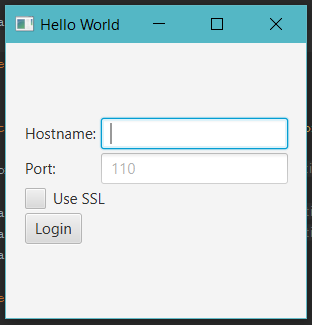
\includegraphics[width=45mm]{img/01_login}
\caption{Pohled přihlášení}
\label{fig:login}
\end{figure}

Po navázání spojení je zobrazen pohled \textbf{Komunikace}, znázorněný Obrázkem \ref{fig:communication}, který umožňuje sledovat a ovlivňovat komunikaci.
V tomto pohledu je výčet zpráv protokolu s nápovědami pro jejich argumenty.
Dále je v tomto pohledu textové pole zobrazující veškerou komunikaci pomocí otevřeného spojení a pole pro zadávání příkazů.

\begin{figure}[h]
	\centering
	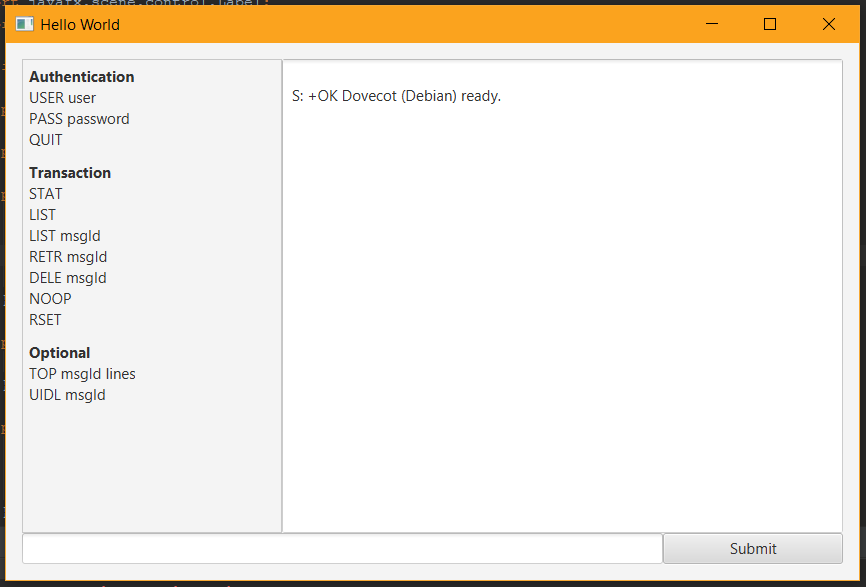
\includegraphics[width=120mm]{img/02_runtime}
	\caption{Pohled Komunikace}
	\label{fig:communication}
\end{figure}

Po zjištění ukončení spojení, respektive po kladné odpovědi na příkaz QUIT, je pole pro zadávání příkazů nahrazeno tlačítkem pro návrat do pohledu \textbf{Přihlášení}.

\section{Implementace}



\subsection{Použití}


\begin{figure}

\end{figure}

\section{Závěr}
Výsledkem této semestrální práce je všeobecně použitelný procházeč SNMP tabulek a podklady pro jednoduché vytvoření nástroje pro práci se SNMP.


%------------------------------------------

\end{document}
